\documentclass[a4paper, 15pt, oneside]{article}
\linespread{1.15} %interlinea
\pagestyle{plain}
\usepackage{geometry} %margini
\usepackage[]{tabto}
\geometry{a4paper, top=3cm, bottom=3cm, left=3cm, right=3cm, bindingoffset=5mm}
\usepackage{graphicx}
\graphicspath{Documentazione/Immagini/}
\usepackage{multicol} %più colonne
\usepackage{ragged2e} %allineamento testo
\usepackage{float}
\author{Gioele Manzoni}
\title{Documentazione per Progettazione Base di Dati}
\begin{document}
	\begin{center}
		\begin{figure}[hb]
			
\includegraphics[width=1\textwidth]{../Immagini/coverpic}
		\end{figure}
		{\LARGE DOCUMENTAZIONE PER PROGETTAZIONE \\ OBJECT ORIENTATION \par}
		{\Large{Progetto in Carico: Hackathon \par}}
		\vfill
		{\large{ \textbf{\textsc{CdL Triennale in Informatica}}}}\\
		{\large{\textsc{Corso di Object Orientation}}}\\
		{\large{\textsc{GIOELE MANZONI}}}\\
		{\large{\textsc{N86004562}}}\\
		{\large{\textsc{LUCA LUCCI}}}\\
		{\large{\textsc{N86005180}}}\\
		{\large{\textsc{\today}}}\\
		\Large{\textsc{Anno Accademico: 2024/2025}}
	\end{center}
	\newpage
	\tableofcontents
	\newpage
	\section{Traccia Progetto: Hackathon}
	Un Hackathon, ovvero una "maratona di hacking", è un evento durante il quale team di partecipanti si sfidano per progettare e implementare nuove soluzioni basate su una certa tecnologia o mirate a un certo ambito applicativo. 
	Ogni Hackathon ha un titolo identificativo, si svolge in una certa sede e in un certo intervallo di tempo (solitamente 2 giorni) e ha un organizzatore specifico (registrato alla piattaforma). L'organizzatore seleziona un gruppo di giudici (selezionati tra gli utenti della piattaforma, invitandoli). Infine, l'organizzatore apre le registrazioni, che si chiuderanno 2 giorni prima dell'evento. Ogni evento avrà un numero massimo di iscritti e una dimensione massima del team.
	Durante il periodo di registrazione, gli utenti possono registrarsi per l'Hackathon di loro scelta (eventualmente registrandosi sulla piattaforma se non lo hanno già fatto). Una volta iscritti, gli utenti possono formare team. I team diventano definitivi quando si chiudono le iscrizioni. All'inizio dell'hackathon, i giudici pubblicano una descrizione del problema da affrontare. 
	Durante l'hackathon, i team lavorano separatamente per risolvere il problema e devono caricare periodicamente gli aggiornamenti sui "progressi" sulla piattaforma come documento, che può essere esaminato e commentato dai giudici. Alla fine dell'hackathon, ogni giudice assegna un voto (da 0 a 10) a ciascun team e la piattaforma, dopo aver acquisito tutti i voti, pubblica le classifiche dei team.
	\section{Analisi Dominio del Problema}
	\subsection{Ricerca delle Classi}
	Le classi trovate sono le seguenti:
	\begin{itemize}
		\item \textbf{Hackathon}: Classe dedicata agli eventi organizzati. Ciascuna sua istanza conterrà le informazioni dell'evento che rappresenterà e sarà di vitale importanza per il funzionamento della struttura.
		\item \textbf{Utente}: Classe per gli Utenti registrati alla piattaforma di organizzazione per gli eventi. Gli Utenti registrati avranno la possibilità di accedere alle varie funzionalità della piattaforma, a seconda dei poteri che gli verranno assegnati.
		\item \textbf{Organizzatore}: Classe rappresentante gli Utenti in grado di organizzare eventi.
		\item \textbf{Giudice}: Classe rappresentante gli Utenti invitati a fare da Giudici per i progetti proposti dai Team delle Hackathon.
		\item \textbf{Team}: Classe che aggrega i partecipanti di un Hackathon. Questa classe farà da portale per tutte le azioni relate alle attività dell'Hackathon alla quale il Team è stato iscritto.
		\item \textbf{Documento}:  Classe per le documentazioni rilasciate dai Team durante lo sviluppo del progetto.
	\end{itemize}
	\newpage
	\subsection{Ricerca Attributi e Associazioni}
		\begin{table}[H]
			\begin{tabular}{lllllll}
				\cline{1-3}
				\multicolumn{3}{|c|}{\textbf{Hackathon}}                                                                                                                                                                                                                        &  &  &  &  \\ \cline{1-3}
				\multicolumn{1}{|c|}{\textbf{Attributo}}      & \multicolumn{1}{c|}{\textbf{Tipo Attributo}}                   & \multicolumn{1}{c|}{\textbf{Descrizione}}                                                                                                      &  &  &  &  \\ \cline{1-3}
				\multicolumn{1}{|l|}{idNum}                   & \multicolumn{1}{l|}{String}                                    & \multicolumn{1}{l|}{Numero identificativo per l'istanza di Hackathon}                                                                          &  &  &  &  \\ \cline{1-3}
				\multicolumn{1}{|l|}{sede}                    & \multicolumn{1}{l|}{String}                                    & \multicolumn{1}{l|}{Sede di appartenenza dell'evento}                                                                                          &  &  &  &  \\ \cline{1-3}
				\multicolumn{1}{|l|}{dataInizio}              & \multicolumn{1}{l|}{String}                                    & \multicolumn{1}{l|}{Data di inizio dell'evento}                                                                                                &  &  &  &  \\ \cline{1-3}
				\multicolumn{1}{|l|}{dataFine}                & \multicolumn{1}{l|}{String}                                    & \multicolumn{1}{l|}{Data della fine dell'evento}                                                                                               &  &  &  &  \\ \cline{1-3}
				\multicolumn{1}{|l|}{dataInizioRegistrazioni} & \multicolumn{1}{l|}{String}                                    & \multicolumn{1}{l|}{Data in cui iniziano le registrazioni all'evento}                                                                          &  &  &  &  \\ \cline{1-3}
				\multicolumn{1}{|l|}{dataFineRegistrazioni}   & \multicolumn{1}{l|}{String}                                    & \multicolumn{1}{l|}{Data in cui finiscono le registrazioni all'evento}                                                                         &  &  &  &  \\ \cline{1-3}
				\multicolumn{1}{|l|}{titolo}                  & \multicolumn{1}{l|}{String}                                    & \multicolumn{1}{l|}{\begin{tabular}[c]{@{}l@{}}Titolo dell'evento descrivente il tema \\ sulla quale i team lavoreranno\end{tabular}}          &  &  &  &  \\ \cline{1-3}
				\multicolumn{1}{|l|}{maxMembriTeam}           & \multicolumn{1}{l|}{int}                                       & \multicolumn{1}{l|}{Numero massimo di membri per team}                                                                                         &  &  &  &  \\ \cline{1-3}
				\multicolumn{1}{|l|}{maxNumIscritti}          & \multicolumn{1}{l|}{int}                                       & \multicolumn{1}{l|}{Numero massimo di iscritti per evento}                                                                                     &  &  &  &  \\ \cline{1-3}
				\multicolumn{1}{|l|}{descrizioneProblema}     & \multicolumn{1}{l|}{String}                                    & \multicolumn{1}{l|}{Descrizione del problema da risolvere}                                                                                     &  &  &  &  \\ \cline{1-3}
				\multicolumn{1}{|l|}{giudiciEvento}           & \multicolumn{1}{l|}{ArrayList\textless{}Giudice\textgreater{}} & \multicolumn{1}{l|}{\begin{tabular}[c]{@{}l@{}}Lista dei giudici che saranno invitati \\ per suddetto ruolo all'Hackathon scelta\end{tabular}} &  &  &  &  \\ \cline{1-3}
			\end{tabular}
		\end{table}
		\begin{table}[H]
			\begin{tabular}{lllllll}
				\cline{1-3}
				\multicolumn{3}{|c|}{\textbf{Utente}}                                                                                                   &  &  &  &  \\ \cline{1-3}
				\multicolumn{1}{|c|}{\textbf{Attributo}} & \multicolumn{1}{c|}{\textbf{Tipo Attributo}} & \multicolumn{1}{c|}{\textbf{Descrizione}}     &  &  &  &  \\ \cline{1-3}
				\multicolumn{1}{|l|}{login}              & \multicolumn{1}{l|}{final String}            & \multicolumn{1}{l|}{Nome utente per il login} &  &  &  &  \\ \cline{1-3}
				\multicolumn{1}{|l|}{password}           & \multicolumn{1}{l|}{String}                  & \multicolumn{1}{l|}{Password dell'utente}     &  &  &  &  \\ \cline{1-3}
			\end{tabular}
		\end{table}
		\begin{table}[H]
			\begin{tabular}{lllllll}
				\cline{1-3}
				\multicolumn{3}{|c|}{\textbf{Organizzatore}}                                                                                                                                   &  &  &  &  \\ \cline{1-3}
				\multicolumn{1}{|c|}{\textbf{Attributo}}   & \multicolumn{1}{c|}{\textbf{Tipo Attributo}}                             & \multicolumn{1}{c|}{\textbf{Descrizione}}              &  &  &  &  \\ \cline{1-3}
				\multicolumn{1}{|l|}{hackathonOrganizzate} & \multicolumn{1}{l|}{private ArrayList\textless{}Hackathon\textgreater{}} & \multicolumn{1}{l|}{Lista delle Hackathon organizzate} &  &  &  &  \\ \cline{1-3}
			\end{tabular}
		\end{table}
		\begin{table}[H]
			\begin{tabular}{lllllll}
				\cline{1-3}
				\multicolumn{3}{|c|}{\textbf{Giudice}}                                                                                                                                                                   &  &  &  &  \\ \cline{1-3}
				\multicolumn{1}{|c|}{\textbf{Attributo}} & \multicolumn{1}{c|}{\textbf{Tipo Attributo}} & \multicolumn{1}{c|}{\textbf{Descrizione}}                                                                            &  &  &  &  \\ \cline{1-3}
				\multicolumn{1}{|l|}{userGiudice}        & \multicolumn{1}{l|}{Utente}                  & \multicolumn{1}{l|}{\begin{tabular}[c]{@{}l@{}}Utente che ha ricevuto l'invito per diventare Giudice\end{tabular}} &  &  &  &  \\ \cline{1-3}
			\end{tabular}
		\end{table}
		\begin{table}[H]
			\begin{tabular}{lllllll}
				\cline{1-3}
				\multicolumn{3}{|c|}{\textbf{Team}}                                                                                                                                                                                                                                                                                             &  &  &  &  \\ \cline{1-3}
				\multicolumn{1}{|c|}{\textbf{Attributo}}   & \multicolumn{1}{c|}{\textbf{Tipo Attributo}}                     & \multicolumn{1}{c|}{\textbf{Descrizione}}                                                                                                                                                                       &  &  &  &  \\ \cline{1-3}
				\multicolumn{1}{|l|}{membro}               & \multicolumn{1}{l|}{Utente{[}{]}}                                & \multicolumn{1}{l|}{\begin{tabular}[c]{@{}l@{}}Lista di Utenti appartenenti al team;\\ Poiché sapremo in anticipo quanto saranno grandi i team,\\ verranno gestiti con l'ausilio di Array statici\end{tabular}} &  &  &  &  \\ \cline{1-3}
				\multicolumn{1}{|l|}{nomeTeam}             & \multicolumn{1}{l|}{String}                                      & \multicolumn{1}{l|}{Nome del team}                                                                                                                                                                              &  &  &  &  \\ \cline{1-3}
				\multicolumn{1}{|l|}{eventoPartecipazione} & \multicolumn{1}{l|}{Hackathon}                                   & \multicolumn{1}{l|}{Hackathon per la quale il team sarà iscritto}                                                                                                                                               &  &  &  &  \\ \cline{1-3}
				\multicolumn{1}{|l|}{documentazione}       & \multicolumn{1}{l|}{ArrayList\textless{}Documento\textgreater{}} & \multicolumn{1}{l|}{\begin{tabular}[c]{@{}l@{}}Lista di tutti i documenti rilasciati dal team durante\\ lo sviluppo del progetto\end{tabular}}                                                                  &  &  &  &  \\ \cline{1-3}
				\multicolumn{1}{|l|}{votoFinale}           & \multicolumn{1}{l|}{int}                                         & \multicolumn{1}{l|}{\begin{tabular}[c]{@{}l@{}}Somma di tutti i voti attribuiti al team \\ alla fine dell'evento\end{tabular}}                                                                                  &  &  &  &  \\ \cline{1-3}
				\multicolumn{1}{|l|}{index}                & \multicolumn{1}{l|}{int}                                         & \multicolumn{1}{l|}{\begin{tabular}[c]{@{}l@{}}Indice di controllo per la grandezza dell'array\\ di membri del team\end{tabular}}                                                                               &  &  &  &  \\ \cline{1-3}
			\end{tabular}
		\end{table}
		\begin{table}[H]
			\begin{tabular}{lllllll}
				\cline{1-3}
				\multicolumn{3}{|c|}{\textbf{Documento}}                                                                                                                                                                  &  &  &  &  \\ \cline{1-3}
				\multicolumn{1}{|c|}{\textbf{Attributo}} & \multicolumn{1}{c|}{\textbf{Tipo Attributo}} & \multicolumn{1}{c|}{\textbf{Descrizione}}                                                                       &  &  &  &  \\ \cline{1-3}
				\multicolumn{1}{|l|}{text}               & \multicolumn{1}{l|}{String}                  & \multicolumn{1}{l|}{Testo della documentazione}                                                                 &  &  &  &  \\ \cline{1-3}
				\multicolumn{1}{|l|}{source}             & \multicolumn{1}{l|}{Team}                    & \multicolumn{1}{l|}{\begin{tabular}[c]{@{}l@{}}Collegamento al team che ha scritto\\ il documento\end{tabular}} &  &  &  &  \\ \cline{1-3}
			\end{tabular}
		\end{table}
	\subsection{Ricerca delle Generalizzazioni}
	\subsection{Ricerca delle Responsabilità}
	\newpage
	\subsection{Grafico UML del Dominio del Problema}
	\begin{figure}[H]
		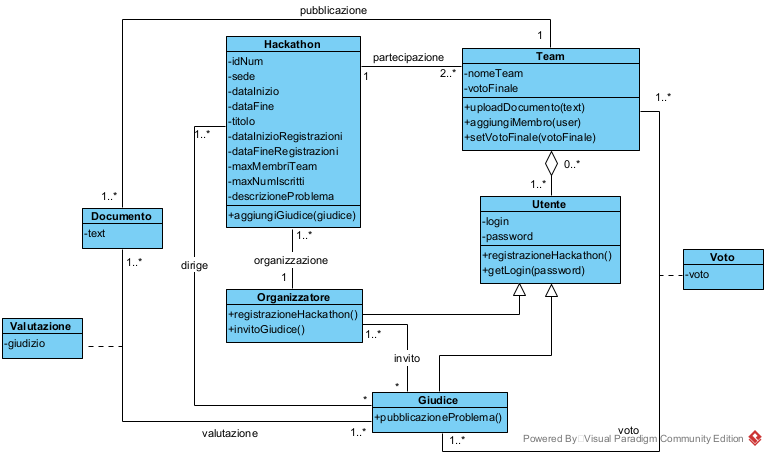
\includegraphics[width=1\textwidth]{../Immagini/Homework1_UMLObject}
	\end{figure}
	
\end{document}
